\documentclass{article}
\usepackage[utf8]{inputenc}
\usepackage{booktabs}
\usepackage{graphicx}
\usepackage[section]{placeins}
\renewcommand{\thesubsection}{\thesection.\alph{subsection}}
\usepackage{natbib}
\title{Tarea 2: Modelo Entidad – Relación }
\author{Arteaga Hernández Alejandro Iabin \and
Barocio Gomez Luis Fernando \and
Castrejón Estrada Juan Carlos \and
Ledesma Granados Roberto Andrés }

\date{Marzo 2020}

\begin{document}

\maketitle

\section{Repaso de conceptos generales}
\subsection{}
Un conjunto de entidades o tipo entidad es un conjunto de entidades
que comparten las mismas propiedades.
- Los tipos de entidad se describen a partir de los metadatos.
Ejemplos: conjuntos de empleados, compañías, clientes, autos, etc.
\par
Podría definirse como una clase, es el conjunto de propiedades que definen a una entidad.
\par\null\par
Una instancia de entidad representa una sola ocurrencia de un tipo de entidad.
Por ejemplo un objeto en java es una instancia de una clase.  \\
Por ejemplo mi perro Cerbero es una instancia del tipo perro.
\subsection{}
Por ejemplo cuando es una relación 1:1 o 1:N
Se pone el atributo en la entidad  contraria al que tiene la cardinalidad 1, por ejemplo\par
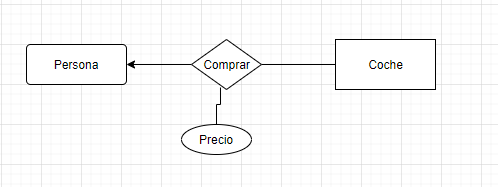
\includegraphics[scale=1]{precio.PNG}
\\Una persona puede comprar varios coches, pero un coche solo puede ser comprado por una persona, el atributo precio, puede ser traspasado a la entidad coche, osea la entidad contraria al que tiene la cardinalidad 1, si los 2 tienen cardinalidad 1, entonces en cualquiera.
\subsection{}

Los relaciones recursivas son relaciones binarias que conectan una entidad consigo
misma.\par\null\par
Por ejemplo una persona que está casada con
otra persona, en la base de datos del registro civil por ejemplo.\par\null\par
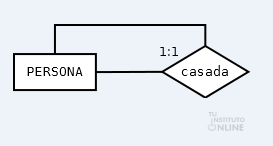
\includegraphics{rec.png}\par\null\par
Un empleado que supervisa a otro empleado, y está almacenado en la misma tabla.\par\null\par
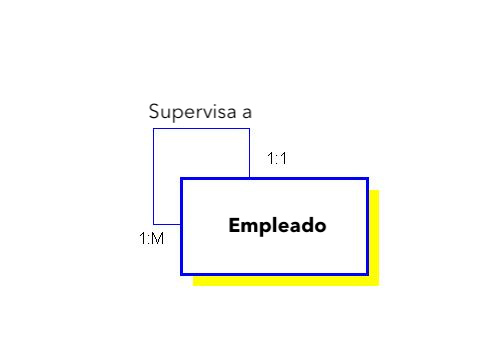
\includegraphics[scale=0.5]{recursiva.jpg}

\subsection{}
\begin{itemize}
    \item ¿Un atributo compuesto puede ser llave?\\\\
    Podría, si el atributo compuesto es único y no nulo, pero no es recomendable porque violaría la primera forma normal.
    \item ¿Un atributo multivaluado puede ser llave?\\\\
    No porque las llaves deben ser únicas para cada fila. y los atributos multivaluados pueden tener varios valores
    \item ¿Un atributo
    derivado puede ser llave?
    \\\\No por definición, la llave primaria no depende funcionalmente de ningún otro atributo y un atributo derivado depende funcionalmente de otro.
    \item ¿Un atributo multivaluado puede ser compuesto?\\\\Sí, por ejemplo, los nombres falsos de un criminal, pero no es recomendable.
    \item ¿Un atributo multivaluado puede ser derivado? \\\\Si, por ejemplo el tiempo de trabajo, si el empleado trabaja en varios departamentos.
    \item ¿Qué implicaría la existencia de una entidad cuyos atributos sean todos derivados?
    \\\\Eso no se podría, ya que se necesita al menos un campo de donde calcular los atributos, y la llave primaria no puede ser calculada porque por definición no depende funcionalmente de ningún otro atributo.
\end{itemize}
\subsection{}
Es un concepto de abstracción para construir objetos compuestos a partir de sus objetos componentes.
\par\null\par
Permite combinar entidades entre las que existe una interrelación y formar una entidad de más alto nivel. Es útil cuando la entidad de más alto nivel se tiene que interrelacionar con otra entidad.
\par\null\par
Ejemplo 1
Se desea almacenar información sobre las entrevistas que una empresa organiza entre solicitantes de empleo y diferentes empresas. Algunas entrevistas dan lugar a ofertas de empleo y otras no.\\
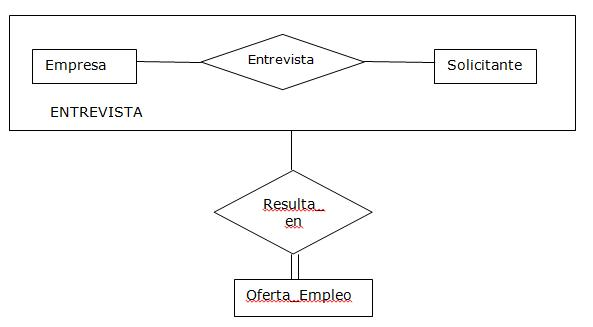
\includegraphics[scale=0.7]{agre.jpg}
\par\null\par
Ejemplo 2:
una nueva entidad ternaria entre Equipos y Empresas, pero esto daría lugar a
redundancia en los atributos de Partido.
Solución: una agregación denominada Partidos, que se tratará como un tipo de entidad y que
puede relacionarse con Empresas. 
\\
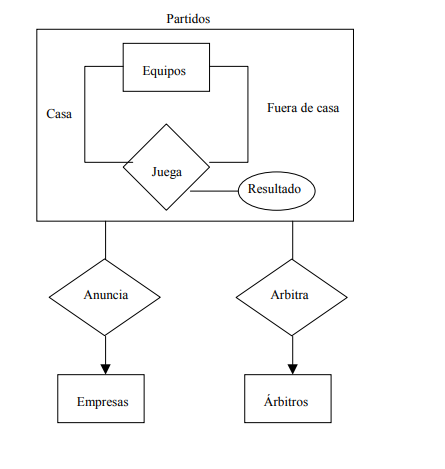
\includegraphics[scale=1]{captura.PNG}
\section{Modelo Entidad/Relación}
\subsection{}
Una persona, tiene que comer uno o más platillos.
Los platillos pueden existir aunque no tengan costo, pueden ser platillos que se dan a empleados.
Pero el precio está en una entidad débil, porque necesita del platillo para poder tener sentido, el costo por si solo no se define. 
Todo precio tiene que venir de un platillo.
\par\null\par
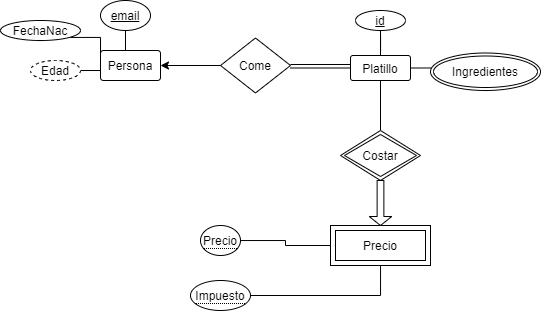
\includegraphics[scale=0.7]{2a.png}
\subsection{}
Consideraciones de diseño\par\null\par
Se decidió hacer la relación operar muchos a muchos con todos los participantes, ya que todos pueden hacerlo varias veces, la única relación a uno es con el obrero, que es el único que repara esa máquina específica, no se usó herencia porque Draw no tenía el símbolo de herencia, pero igualmente el diagrama es válido sin ella.\\
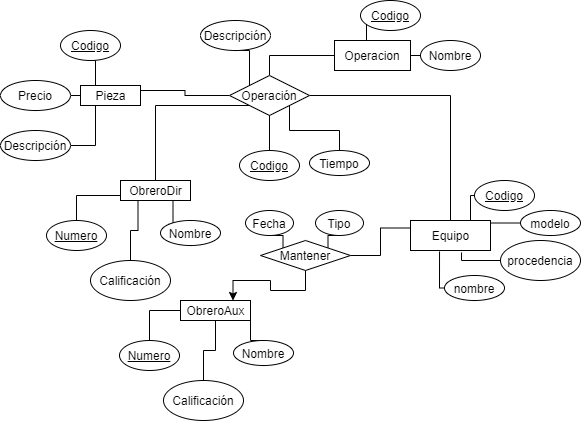
\includegraphics[scale=0.7]{ggg.png}
\subsection{}
Decidimos dejar la relación comprar como muchos a muchos, porque un producto puede ser comprado por muchos clientes, pueden ser vendidos por muchos vendedores. Mientras la cantidad disponible sea mayor a cero, pero eso se verifica con un disparador.
\par\null\par
Mientras que solo se puede adoptar a un perro una vez, entonces solo tiene un cliente y un empleado asignado.
\par\null\par
Ninguna relación es total, porque hay perros no adoptados, hay clientes que no compran solo están registrados, y hay empleados que no venden. 
\par\null\par
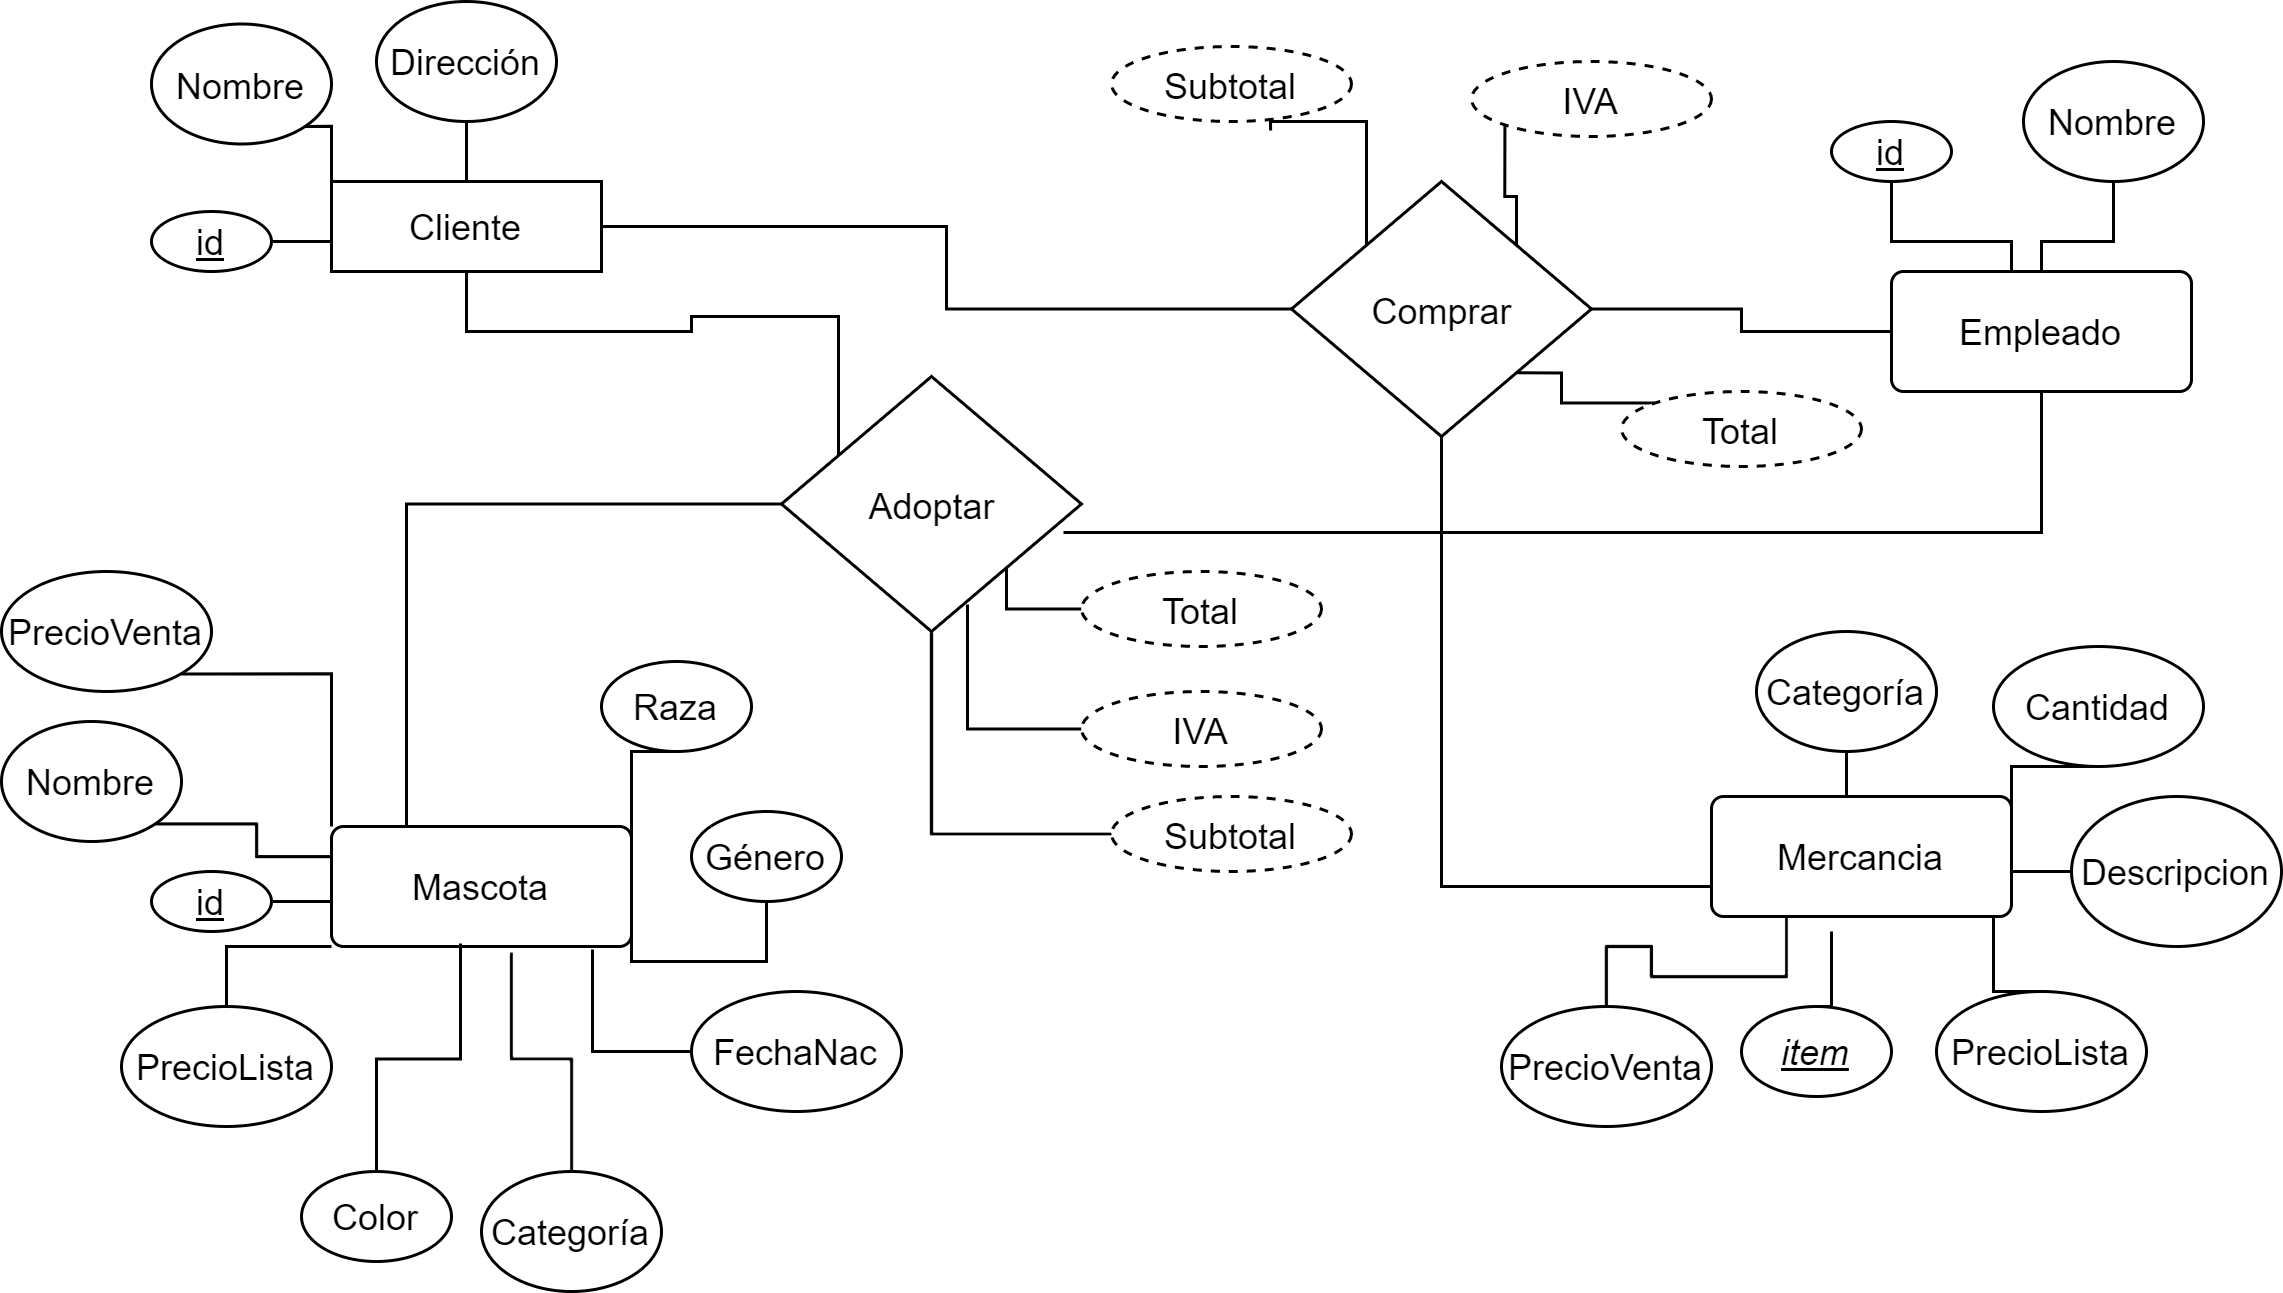
\includegraphics[scale=0.185]{tike.png}
\section{Ingeniería inversa}
\begin{itemize}
    \item En esta base de datos no hay ningún actor que no haya actuado en ninguna película.\par\null\par
    Verdadero, debido a la relación de orden total con la entidad película.
    \item Hay algunos actores que han actuado en más de diez películas.
    \par\null\par
    Verdadero, puede haber actores que hayan participado en n películas.
    \item Algunos actores han sido protagonistas en varias películas.
    \par\null\par Verdadero, un actor puede protagonizar varias películas, la relación es 1:n ya que una película solo puede ser protagonizada por un actor.
    \item Una película sólo puede tener un máximo de dos protagonistas.
    \par\null\par
    Falso, las películas solo pueden ser protagonizadas por un actor.
    \item Cada director ha sido actor en alguna película.
    \par\null\par
    Verdadero, porque todos los directores son actores, entonces como es total la relación actuar, todos los directores han actuado. 
    \item Ningún productor ha sido actor alguna vez.
    \par\null\par Falso, todos los productores son actores.
    \item Un productor no puede ser actor en alguna otra película.
    \par\null\par
    Falso, los productores son actores y por la relación debieron actuar en alguna película.
    \item Hay películas con más de una docena de actores.
    \par\null\par Verdadero, puede haber N actores.
    \item Algunos productores también han sido directores.
    \par\null\par Verdadero, un productor podría ser director también,
    \item La mayoría de las películas tienen un director y un productor.
    \par\null\par
    Falso, todas las películas, deben tener un actor y un productor.
    \item Algunas películas tienen un director, pero varios productores.
    \par\null\par
    Falso, solo puede haber un productor por película.
    \item Hay algunos actores que han interpretado el papel de protagonista, dirigido una película y
    producido alguna película.
    \par\null\par
    Verdadero, un actor puede ser protagonista, director y productor porque la relación de herencia es traspuesta, entonces las entidades, pueden ser padre o hijos o los dos,
    \item Ninguna película tiene un director que también haya actuado en ella.
    \par\null\par
    Falso, un director puede haber actuado en una película.
\end{itemize}
\section{Referencias}
\textbf{$https://virtual.itca.edu.sv/Mediadores/dbd/u1/entidades_dbiles.html$}\par\null\par
\textbf{$http://www.codecompiling.net/files/slides/BD_clase_04_modelo_ERE.pdf$}\par\null\par
\textbf{$https://en.wikipedia.org/wiki/Entity-relationship_model$}
 \end{document}
